%!TEX root = ../Peerbox.tex
Peer-to-peer systems have become most popular recently in social, academic and commercial domains. These systems use networks in which each computer can act as a client or server for other computers without the need of a central server. One of the early driving forces behind peer-to-peer concept is that there are many PC's at home and offices that lie idle for large chunks of time. These resources can be leveraged for content sharing. In this report, we present the design and implementation of a peer-to-peer file sharing system known as \textbf{"Peerbox"}. This project is a part of  \textbf{Distributed Systems} course. This project is mainly targeted for university students who can share their work amoung their group. This system proves helpful in sharing and saving files. It is intended for small groups with an average size of 3-5 members. We identified some major advantages like scalability, performance, heterogeneity while using this system. However there are still some issues like security, mobile transparency, location transparency and replication which will be dealt in future.  


The report is organized in different sections. Section 1 gives a general idea about the working of the Peerbox system.It describes about how file-sharing is done using the technique known as multicasting and introduces some of the most popular peer-to-peer file sharing systems that were developed recently. Section 2 discusses about some scenarios where we get acquainted with the various operations done in a peer-to-peer system.  It also discusses about some important properties of the Peerbox system. Section 3 discusses about the overall design and architecture of the system. It describes each architectural layer in detail. Section 4 discusses about different results achieved by the actual implementation of the Peerbox system.       
\subsection{Idea}
%manni

Christian, Divya and Spyros are three students who work on a project based on Cloud Computing Project. The ideal for them, would be to work together to achieve their goals. This involves sharing their work with each other. However, there may be some situations where internet cannot be accessed, which may in turn delay their project. Nevertheless, the students need to work effectively by sharing their work - this means that they should be able to access files that are stored on another computer. This can be accomplished by combining the computers in a Virtual File System (VFS) that automatically adds files in a peer-to-peer scheme. Hence, the VFS would automatically detect new peers and show their file, so that they can accessed by the group members.

Implementing the proposed solution, would  enable them to work across network boundaries without setting up complex shared folders, creating a flexible file structure and thus the peers do not have to be connected via internet. In this way, every student will not need to transmit ownership of a file because the file is stored locally on his computer File sharing will be possible with minimal configuration. 

 
\begin{figure}[H]
\begin{center}
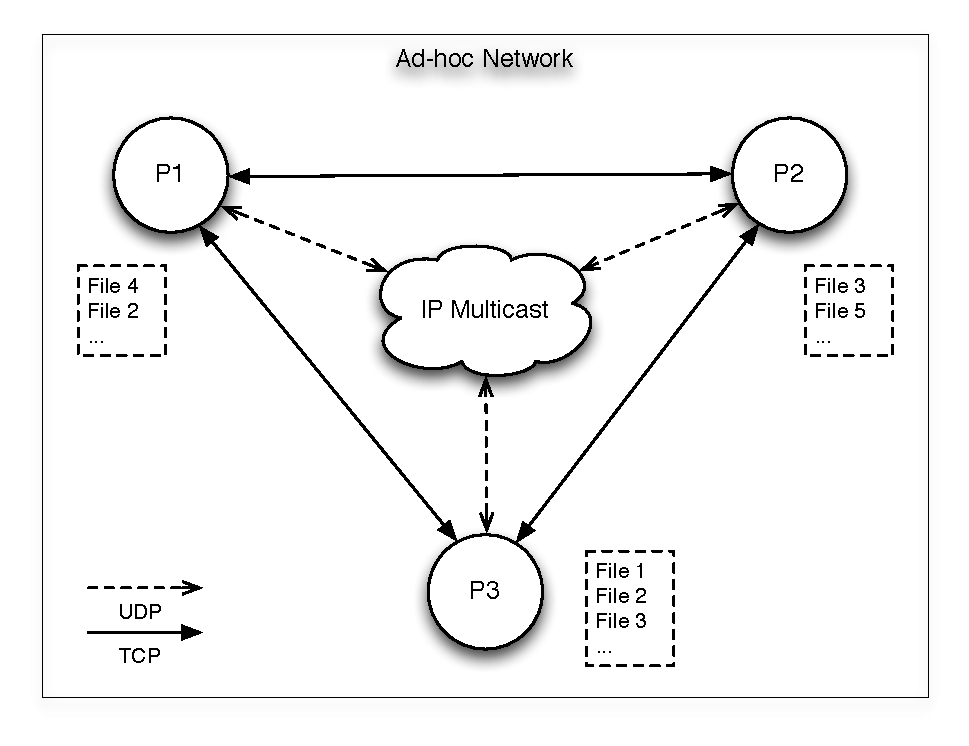
\includegraphics[height=3in]{figures/idea.pdf}
\caption{The high level idea of Peerbox}
\label{fig:idea}
\end{center}
\end{figure}



\subsection{Context}
%manni
The main goal of the Peerbox system is to enable file sharing among different peers. Here, the process of multicasting is used where a set of data packets are transmitted to  multiple hosts who have joined the multicast group simultaneously. 

After joining the group, the peer can request the list of files, create files, update the files as well as delete files.



\section{State of the Art}
%spyros

During the last decade, various peer-to-peer file systems were introduced. Most of them share common properties like availability, sharing, safety and decentralization. However, some more advanced peer-to-peer file systems offer important properties like synchronization and conflict detection. This section provides the state of the art in peer-to-peer file systems.

\begin{description}
	\item[Pastis]\-\\
	Pastis \cite{Busca:2005gt} is a decentralized multi-user read-write peer-to-peer file system. Every file is described by
a modifiable inode-like structure which contains the addresses of the immutable blocks in which the file contents are stored.

All the data is stored using the Past \gls{acr:dht}, which has been modified in order to reduce the number of network messages it generates, thus optimizing replica retrieval. Pastis is known for its simplicity, high scalability, fault tolerance and locality properties of its underlying storage layer.

	\item[Ivy]\-\\
	Ivy \cite{Muthitacharoen:2002iv} is a multi-user read and write peer-to-peer file system. It has no centralized or dedicated components. It provides useful integrity properties without requiring users to fully trust either the underlying peer-to-peer storage or other users of the file system.
	
	One of its important properties is that with a special arrangement between logs and the modifications of participants, it maintains meta-data consistency without locking. Ivy provides semantics like \gls{acr:nfs} and is able of detecting conflicting modifications. Performance measurements show that Ivy is two to three time slower than \gls{acr:nfs}.
	\item[ColonyFs]\-\\
	ColonyFS \cite{Colony:2009fs} is a distributed file system which emphasizes anonymity, security and dependability over a peer to peer network. This system implements a technique called \gls{acr:frs} and uses an optimization algorithm inspired by the movement of ants. The aim of the project is to produce an implementation of these techniques for the specific requirements of a dynamic peer-to-peer network where participants can join and leave at will.
	\item[Infinit]\-\\
	Infinit\footnote{http://en.wikipedia.org/wiki/Infinit} is a peer-to-peer file system which allows users to store, access and share files in a safe and collaborative way. It also allows the virtualization of decentralized storage space as one coherent drive. Infinit ensures reliability by dynamically replicating the data so that devices can crash without incurring data loss. It also ensures privacy by access control mechanisms.
	
	Furthermore, it is known for ensuring synchronization by distributing files and directories throughout the network's infrastructure and update them in real time. Some additional properties of Infinit are sharing, transparency, security, anonymity, and availability.
	\item[Darknet]\-\\
	Darknet \cite{Ledung:2010wq} is private peer-to-peer file system which aims to provide safe, fast, and scalable file sharing without constraining the users in this aspect. It utilizes a decentralized peer-to-peer network overlay by creating a prototype with extreme programming as methodology. To maximize the freedom of users the network is accessed through a virtual file-system interface.
\end{description}
